\documentclass[smallcondensed]{svjour3} 
%\documentclass{sig-alternate}
\usepackage{url}
\usepackage{graphics}
\usepackage{graphicx}
\usepackage{amsmath}
\usepackage{amssymb}
\usepackage{subfigure}
\usepackage{microtype}
%\usepackage{epsfig}
%\usepackage{graphics}
%\usepackage{amsthm}

\newenvironment{xmpl}{\begin{example}\hspace{-.5em} \begin{textit}}{\end{textit}$\Box$\end{example}}

\newcommand{\todo}[1]{{\bf [TODO:{\em {#1}}]}}
\newcommand{\josh}[1]{{\bf [JOSH:{\em {#1}}]}}
\newcommand{\panos}[1]{{\bf [PANOS:{\em {#1}}]}}
\newcommand{\foster}[1]{{\bf [FOSTER:{\em {#1}}]}}
\newcommand{\drop}[1]{}

%\newtheorem{definition}{Definition}
%\newtheorem{example}{Example}
%\newtheorem{theorem}{Theorem}
 
 \begin{document}
 
\title{Beat the Machine: Challenging Humans to Find a Predictive Model's ``Unknown Unknowns''}


\author{Josh Attenberg         \and
        Panagiotis G.\ Ipeirotis \and Foster Provost %etc.
}


%\numberofauthors{3}
%\author{
%\alignauthor
%Josh Attenberg\\
%       \affaddr{New York University}\\
%       \affaddr{Brooklyn, NY} \\
%       \email{josh.attenberg@gmail.com}
%% 2nd. author
%\alignauthor
%Panagiotis G. Ipeirotis\\
%       \affaddr{NYU Stern School of Business}\\
%       \affaddr{New York, NY}\\
%       \email{panos@stern.nyu.edu}
%% 3rd. author
%\alignauthor 
%Foster Provost\\
%       \affaddr{NYU Stern School of Business}\\
%       \affaddr{New York, NY}\\
%       \email{fprovost@stern.nyu.edu}
%}
%
%
%%\authorrunning{Short form of author list} % if too long for running head
%
%\institute{F. Author \at
%              first address \\
%              Tel.: +123-45-678910\\
%              Fax: +123-45-678910\\
%              \email{fauthor@example.com}           %  \\
%%             \emph{Present address:} of F. Author  %  if needed
%           \and
%           S. Author \at
%              second address
%}





\maketitle

\begin{abstract}

We present techniques for gathering data that expose errors of automatic predictive models.  In certain common settings, traditional methods for evaluating predictive models tend to miss rare-but-important errors---most importantly, cases for which the model is confident of its prediction (but wrong).  In this paper, we present a system that, in a game-like setting, asks humans to identify cases that will cause the predictive-model-based system to fail. Such techniques are  valuable in discovering problematic cases that do not reveal themselves during the normal operation of the system, and may include cases that are rare but catastrophic. We describe the design of the system, including design iterations that did not quite work. In particular, the system incentivizes humans to provide examples that are difficult for the model to handle, by providing a reward proportional to the magnitude of the predictive model's error. The humans are asked to ``\emph{Beat the Machine}'' and find cases where the automatic model (``\emph{the Machine}'') is wrong. Experiments show that the humans using Beat the Machine identify more errors than traditional techniques for discovering errors in from predictive models, and indeed, they identify many more errors where the machine is confident it is correct.  Further, the cases the humans identify seem to be not simply outliers, but coherent areas missed completely by the model.  Beat the machine identifies  the ``unknown unknowns.''


\begin{quotation}
\em ``There are known knowns. These are things we know that we know. There are known unknowns. That is to say, there are things that we know we don't know. But there are also unknown unknowns. There are things we don't know we don't know.''\\~\\
-- \textbf{Donald Rumsfeld}
\end{quotation}

\end{abstract}

\section{Introduction}
\label{sec:intro}


Many businesses and government organizations make decisions based on
estimations made by explicit or implicit models of the world.  Being
based on models, the decisions are not perfect.  Understanding the
imperfections of the models is important (i)~in order to improve the
models (where possible), (ii)~in order to prepare to deal with the
decision-making errors, and (iii)~in some cases in order to properly
hedge the risks.  However, a crucial challenge is that, for 
complicated decision-making scenarios, we often do not know where 
models of the world are imperfect and/or how the models' imperfections
will impinge on decision making. \emph{ We don't know what we don't know.}

We see the results of such failures of omniscience in grand
catastrophes, from terrorist attacks to unexpected nuclear disasters,
in mid-range failures, like cybersecurity breaches, and in failures of
operational models, such as predictive models for credit scoring,
fraud detection, document classification, etc.

Unknown unknowns are related to the classic contrast between reasoning
systems that make open- and closed-world
assumptions~\cite{Reiter77closedworld}: are the only answers to a query Q those
that are actually in the database?  In the context of predictive
modeling, in applications with limited labeled training data, small
disjuncts\cite{weiss10disjunct}, and possibly unknown selection biases, are
we willing to make the assumption that regularities that have no or
insufficient representation in the training data essentially do not
exist?

% In the context of data mining, one can
% think of learning methods as implicitly or explicitly making a
% closed-world assumption: 
% Whether
% learning systems truly make a closed-world assumption may be debatable
% under strict assumptions of learning theory and decision theory, where
% training data are sampled from the same population to which the model
% will be applied, and we know the costs of making errors.  However, in
% the real world we often learn and apply models anyway in the face of
% various sampling biases, often that we do not even know about.  Furthermore, 
% as we will describe, we often have 

In this paper we introduce and analyze a crowdsourcing system designed
to help uncover the ``unknown unknowns'' for predictive models.  The
system is designed to apply to settings where assessing the
performance of predictive models is particularly challenging.  Later we
will describe in detail the critical aspects of such settings, but
first let us introduce a motivating example to make the discussion
concrete.

Consider the following task: a firm has built a system for identifying
web pages that contain instances of ``hate speech'' (e.g., racist
content, antisemitism, and so on), based on a model that takes web
pages as input and produces as output a ``hate score.''  The firm
would like to use this system to help protect advertisers, who
(despite the best efforts of their advertising agents) sometimes see
their ads appearing adjacent to such objectionable content.  The
advertisers do not want their brands to be associated with such
content, and they definitely do not want to support such content,
explicitly or implicitly, with their ad dollars.  

How does this firm assess the strengths and weaknesses of its system
and model?  This scenario comprises a constellation of factors that
are not uncommon in organizational decision making, but are quite
problematic for conducting the assessment---particularly because of
the problem of unknown unknowns.  Specifically, this paper considers
applications where:

\begin{itemize}
\itemsep=0.0in
\item Every decision-making case can be represented by a description
  and a target.  We have a (predictive) model that can give us an estimate or
  score for the target for any case.  For this paper, we assume for
  simplicity that the target is binary, and that the truth would not
  be in dispute if known.\footnote{For our example, the
  description of the case would be the web page (its words, links,
  images, metadata, etc.).  The target would be whether or not it
  contains hate speech.}

\item We want to understand the inaccuracies of the
  model---specifically, the errors that it makes, and especially
  whether there are systematic patterns in the errors.  For example,
  is there a particular sort of hate speech that the model builders
  did not consider, and therefore the model misses it?

\item The process that is producing the data does not (necessarily)
  \textit{reveal} the target for free.  In our example, if we
  misclassify a hate speech page as being OK, we may never know.
  (Indeed, we usually never know.)  This is in contrast to
  \textit{self-revealing} processes; for example, in the case of credit-card
  fraud detection, we will eventually will be informed by the customer
  that there is fraud on her account.  For targeted marketing, we
  often eventually know whether the consumer responded to an offer or
  not.

\item Finally, there are important classes or subclasses of cases that
  are very rare, but nevertheless very important.  The rarity often is
  the very reason these cases were overlooked in the design of the
  system.  In our example, hate speech on the web itself is quite
  rare (thankfully).  Within hate speech, different subclasses are
  more or less rare.  Expressions of racial hatred are more common
  than expressions of hatred toward dwarves or data miners (both real cases).

\end{itemize}

These problem characteristics combine to make it extremely difficult to
discover system/model imperfections.  Just running the system, in
vitro or in vivo, does not uncover problems; as we do not observe
the true value of the target, we cannot compare the target to the model's
estimation or to the system's decision.

We \textit{can} invest in acquiring data to help us uncover
inaccuracies.  For example, we can task humans to score random or
selected subsets of cases.  Unfortunately, this has two major
drawbacks.  First, due to the rarity of the class of interest (e.g.,
hate speech) it can be very costly to find very few positive examples,
especially via random sampling of pages.  For example, hate speech
represents far less that $0.1\%$ of the population of web pages, with unusual or distinct forms of hate speech being far rarer still. Thus we would
have to invest in labeling more than 1000 web pages just to get one hate speech
example, and as has been pointed out
recently, often you need more than one label per page to get
high-quality labeling~\cite{shengKDD2008,raykar2009supervised}.


% whatever this means for model
% performance~\cite{forman2006quantifying}


In practice, we often turn to particular heuristics to identify
cases that can help to find the errors of our model.  There has been a
large amount of work studying ``active learning'' which attempts to
find particularly informative examples~\cite{SettlesActiveLearning}.
A large number of these strategies (uncertainty sampling, sampling
near the separating hyperplane, query-by-committee, query-by-bagging,
and others) essentially do the same thing: they choose the cases where
the model is least certain, and invest in human labels for these.
This strategy makes sense, as this is where we would think to find
errors.  Additionally, there has been a long history of understanding that
``near misses'' are the cases to use to best improve a model, both for
machine learning~\cite{winston1970learning} and for human
learning~\cite{vanlehn1998analogy}.

Unfortunately, although helpful in understanding and improving
modeling, for finding unknown unknowns, 
these strategies look exactly where we don't want to look.
These strategies explicitly deal with the ``known unknowns.''  The
model is uncertain about these examples---we ``know'' that we don't
know the answer for them (i.e., we have low confidence in the model's
output).  These strategies explicitly eschew, or in some cases
probabilistically downweight, the cases that we are
certain about, thereby \textit{reducing} the chance that we are going
to find the unknown unknowns.

With that substantial preamble, we can now state succinctly the goal
and contributions of this paper.  First, we describe the problem more
formally, including relationships to prior work.  We next discuss
changes to how we need to view the evaluation of classifiers, if we
want to move from a closed-world view of a predictive modeling problem
to an open-world view.  Then we introduce a technique and system to use
human workers to help find the \emph{unknown unknowns}.  Our
BeatTheMachine (BTM) system combines a game-like setup with incentives
designed to elicit cases where the model is confident and wrong.
Specifically, BTM rewards workers that discover cases that cause the
system to fail. The reward increases with the magnitude of the
failure. This setting makes the system to behave like a game,
encouraging steady, accurate participation in the tasks. We describe
our first experiences by the live deployment of this system, in a
setting for identifying web pages with offensive content on the
Internet. We show that this BTM setting discovers cases that are
inherently different than the errors identified by a random sampling
process. In fact, the two types of errors are very different. The BTM
process identifies ``big misses'' and potential catastrophic failures,
while traditional model-based example selection identifies ``near
misses'' that are more appropriate for fine-tuning the system.  The
evidence shows that BTM does not just find individual ``oddball''
outlier cases, but it finds systematic big errors.  In a sense, the
BTM process indeed gives us the opportunity to learn our ``unknown
unknowns'' and warn us about the failures that our current automatic
model cannot (yet) identify by itself.



\input{2-background.tex}
\section{Unknown Unknowns}
\label{sec:unknowns}

In order to provide a detailed discussion of unknown unknowns in the context of a predictive model, it is first necessary to formalize the concepts we will be discussing. Let $x$ represent an example belonging to some problem space $X$. In classification settings, $x$ has a ``true'' label, $\bar{y}$ from some set of possible labels $Y$. The task of a classification is to construct some predictive model, $f(x)$, that can estimate a label for each incoming example ($y = f(x)$) such that the estimated label $y$ mirrors the (usually hidden) true label, $\bar{y}$, as closely as possible. There is a cost $c_{ij}$ for a misclassification decision, when we classify an example from the true category $\bar{y}=y_i$ into a category $f(x)=y_j$. In this work, we are concerned only with models that output a posterior probability estimate over the set of available labels, that is, $f(x) = p(y | x) = \langle p_1, \ldots, p_n \rangle$; such models, through the probability estimates, effectively also  report the estimated misclassification cost of each example:

\begin{eqnarray}
\widehat{\mathit{ExpCost}}(x) & = & \sum_{i,j} p_i \cdot p_j \cdot c_{ij} \label{equ:expcost} \\
\widehat{\mathit{MinCost}}(x) & = & \mbox{min}_j \sum_{i} p_i \cdot c_{ij} \label{equ:mincost}
\end{eqnarray}

Such probabilities can then be used to select a preferred label, for instance by choosing the $y$ with the highest probability, or in the cost-sensitive setting, choosing the label with the least expected cost~\cite{elkan:2001cost}. Note that the focus on models that produce probability estimates is without loss of generality--- there exists a variety of techniques for transforming ``hard-labeling'' models into probability estimators (see, eg.~\cite{domingos1999metacost, Platt99probabilisticoutputs}).

Notice that Equations~\ref{equ:expcost} and~\ref{equ:mincost} provide \emph{estimates} of the misclassification cost. The \emph{actual} misclassification cost can be different and depends on the accuracy of the model and the generated posterior probability estimates. The difference between the estimated and the 
actual misclassification costs gives birth to four different types of data points, as depicted in Figure~\ref{fig:quadrant}.

\begin{figure}[t]
\centering
\includegraphics[width=0.5\columnwidth]{plots/Quadrant.png}
\caption{The decisions made by a predictive model can be broadly separated into four conceptual regions: (i)~The ``known knowns,'' which are the examples for which the model is mostly correct and is also confident of being correct; (ii)~The ``known unknowns,'' which are the examples for which the model is often mistaken but also anticipates these mistakes by placing low confidence in the decisions; (iii)~The ``unknown knowns,'' which are the examples for which the model is often correct but returns very low levels of confidence; and (iv)~The ``unknown uknowns,'' which are the examples for which the model is wrong but also confident on being correct.}
\label{fig:quadrant}
\end{figure}

Along the diagonal, we have examples, for which the estimates of the model in terms of misclassification cost are in line with the actual classification costs. In the lower-left corner we have the examples that the model can classify correctly \emph{and} is confident about the reported decisions. These are the ``\emph{known knowns}''. In the upper-right corner, we have the cases of ``known unknowns'': these are the cases where the model fails often but is also aware about this problem.

\begin{definition}[Known Unknown]
\label{def:ku}
Let $X' \subset X$ be a region of the problem space and $x$ be a randomly picked example from $X'$. 
We denote by $\widehat{\mathit{ExpCost}}(X')$ the expected misclassification cost of the examples in $X'$, and $\mathit{ExpCost}(X')$ be the actual misclassification cost of the examples in $X'$. A \emph{known unknown} is an example for which the actual misclassification cost $\mathit{ExpCost}(x)$ is high \emph{and} the estimated misclassification cost $\mathit{ExpCost}(X')$ is also high.
\end{definition}

Known unknowns as described in Definition~\ref{def:ku} corresponds to a commonly occurring notion in machine learning. The $X'$ region corresponds to an ``uncertainty'' region, an area where the predictive model is unsure of itself, and where mistakes are likely. This concept has been exploited in a variety of contexts, for instance, when applied to the problem of gathering labels for the purpose of model training, selecting those examples within an $\epsilon$-radius of the decision boundary corresponds to uncertainty sampling, perhaps the most well known active learning heuristic~\cite{lewis94sequential}.

In the context of prediction-time classification, ``known unknowns'' are those cases for which errors are expected based on the confidence of the classification.   These are cases where it may be less costly to ``reject'' than to make a risky label prediction.  Classification with a ``reject option'' is an extension of traditional classification where in addition to labeling each example with some $y \in Y$, a predictive system may additionally defer prediction, either by ignoring an example entirely, or perhaps sending the example to a domain expert for manual evaluation~\cite{chow:57,chow:70}. Given that such ``rejection'' likely comes at some non-trivial cost $q(x)$, the task of classification with a reject option is then to balance the expected misclassification costs with the costs of rejection.  Appendix~\ref{app:reject} presents the ideas of classification with a reject option in detail, as they relate closely to the notion of a known unknown.

While it is important to understand the mistakes that your model is known to make and to react in an appropriate manner, models in production often make mistakes far from this area of predicted uncertainty. Consider the hate speech classification system discussed previously. While deployed in a production setting, this model is likely to encounter examples eliciting a high degree of predicted uncertainty.\footnote{For instance, a encyclopedia entry discussing racial issues or a history of racism.} Those managing the model can react to these borderline examples, and perhaps build some rough estimate of a model's overall exposure to misclassification risk. However, for a variety of reasons, the model may also encounter examples where it will assign a label with high confidence, and be wrong. Call all such examples ``unknown unknowns.''

\begin{definition}[Unknown Unknown]
\label{def:uu}
Following Definition~\ref{def:ku}, an example $x'$ is said to be an ``\emph{unknown unknown}'' if $x'$ is outside the region of uncertainty and has \emph{low} estimated misclassification cost $\widehat{\mathit{ExpCost}}(X')$, but the actual misclassification cost $\mathit{ExpCost}(x)$ is high. In other words, the example is misclassified but the classifier is certain that it was correctly classified.
\end{definition}

Definition~\ref{def:uu} codifies the notion of an ``unknown unknown''. Intuitively, these are examples that are distant from any decision boundary, examples that the model is quite certain a correct label can be assigned, yet are still labeled incorrectly.  While in the strict sense, the above definition includes ``random noise''---individual examples that for whatever reason do not have the expected label,\footnote{For instance,  due to erroneous labeling, signal degradation, or non-pathological difficulties in data collection.}---the motivating case is disjunctive sub-regions of the problem space~\cite{weiss10disjunct}. These are small, yet consistently labeled neighborhoods of examples isolated from the body of examples of the same class. These ``islands'' of examples may be sufficiently rare in the relative sense to avoid detection from random sampling processes used to generate training sets~\cite{attenberg:2010inactive, attprov:kdd2010}. However, their absolute size and prevalence in many real world problems makes them a genuine risk.

Figure~\ref{fig:unknown} presents a fairly typical classification
scenario that might be impacted by ``unknown unknowns''. On the top,
we see an inseparable two-class problem, with a linear decision
boundary that minimizes the prediction errors on this space. Above and
below this decision boundary, we see an a region of uncertainty, $\epsilon$-wide,
where mistakes are \emph{known} to occur. This
represents a typical post-training understanding of the problem space: 
data is gathered by some random process, for instance via active
learning. An imperfect model is trained, however, areas where mistakes
occur are known and expectations can be managed. On the bottom we see
a typical scenario when such models are deployed in the wild---rare
disjunctive sub-regions of the problem space emerge.  These are portions of the
problem space that escaped the initial sampling process used to generate
the training set. These unknown unknowns while small in terms of their
proportion of the problem space may still exist in large absolute
numbers.  However, because they are unobserved during model
construction, they have likely escaped any possible contingency
planning for dealing with their associated mistakes.

\begin{figure}[t]

\begin{center}
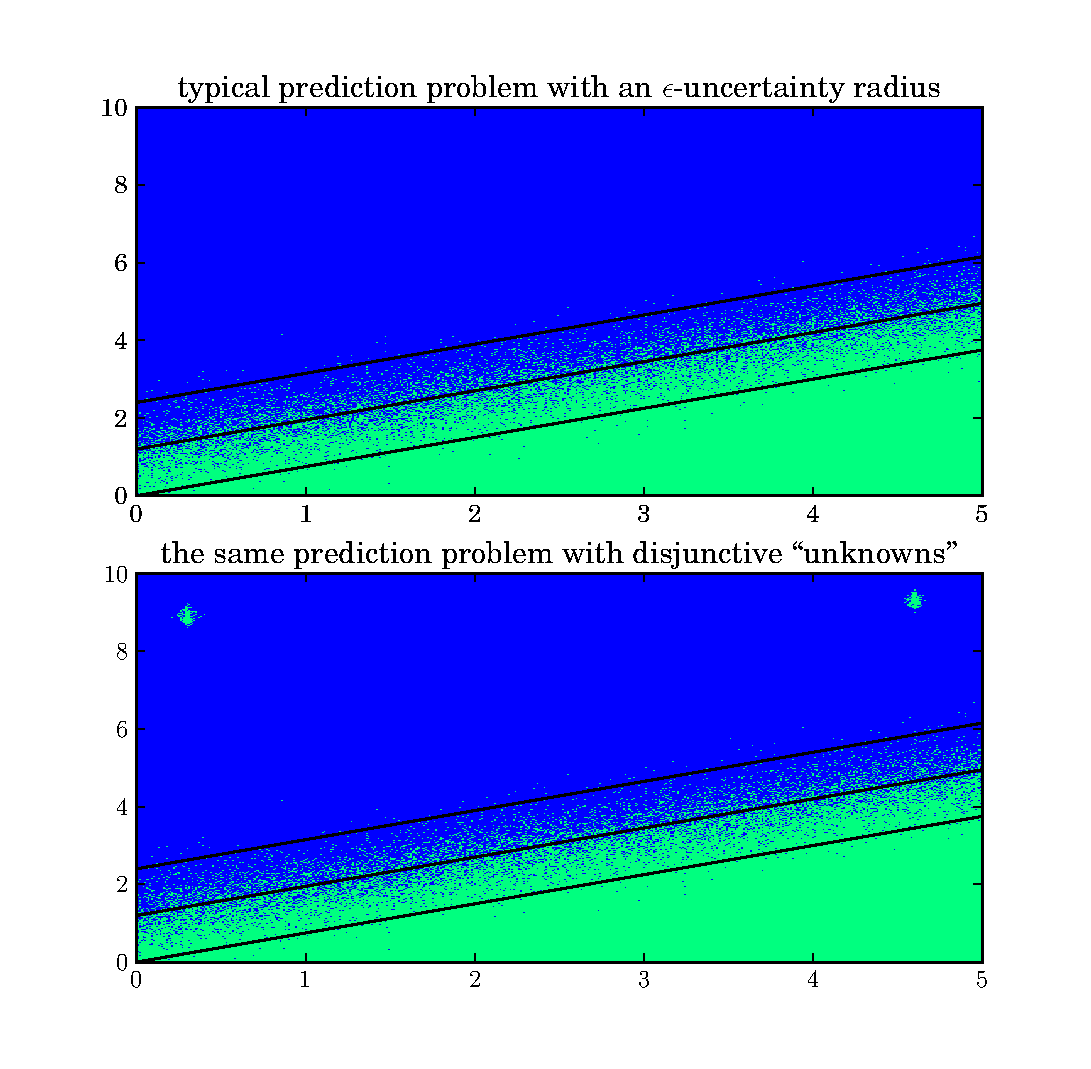
\includegraphics[width=0.6\columnwidth]{plots/example_function_2.png}
\end{center}
\caption{A typical classification setting. On the the top we see the decision boundary that minimizes the prediction prediction error of a inseparable training set. Additionally, we see the $\epsilon$-radius around the classifier where mistakes are though to occur. The bottom, we see the same classifier with the inclusion of small, disjunctive ``unknowns'', presenting mistakes that occur well outside a model's region of uncertainty. }
\label{fig:unknown}
\end{figure}

Finally, from Figure~\ref{fig:quadrant}, we can see that there is one more type of examples: The ``\emph{unknown knowns}''. These are the cases where the model is incorrectly pessimistic: The model reports low confidence and high estimated cost for the examples in these region(s). However, in reality the model generates mostly correct predictions. Such cases are typically easier to manage but may still cause problems in the stakeholders: if this region generates many rejects (with an associated inspection and intervention costs), then the model will be perceived as being overly cautious and potentially inefficient. Despite the fact that it is a promising direction, identifying and dealing with cases of unknown knowns is beyond the scope of this paper, and we leave their study for future work.
\section{Measuring Unknown Unkowns}
\label{sec:measure}

This section attempts to quantify the tradeoffs associated with
unknown unknowns faced by predictive modeling systems.  Prudence dictates that any
predictive model should be evaluated thoroughly in a lab before
deployment into the wild. However, because perfect predictive
performance is rarely achieved in practice, a model's manager often
needs to be concerned with the cases that the model deems to be
uncertain.  The uncertainty radius $\epsilon$ is a theoretical
construct representing the cases of concern: those for which the model
is too uncertain and returns a higher estimated misclassification cost. 
A higher uncertainty radius reduces the chance of the model encountering ``unknown unknowns,'' but
 presumably there is an increased cost incurred to deal with these cases, increasing the number of ``unknown knowns.''
The cases could be rejected from automatic processing, and sent to
humans (cf., the setting of classification-with-a-reject option setting discussed above), or the
cases may get extra-close monitoring, or customer-expectations may be
lowered, etc.  On the other hand, a lack of concern may result in
unmitigated mistakes, which may induce cost beyond that enumerated in
a problem's formal loss structure due to a lack of preparation and contingency
planning.

Figure~\ref{fig:uuvsku} presents example curves showing the tradeoffs
between the percentage of cases lying inside a model's
$\epsilon$-radius uncertainty bounds, where the model reports high estimated misclassification costs, 
and the number of unmitigated
mistakes (unknown unknowns) made by that model, considering the same
problem presented in Figure~\ref{fig:unknown}.  Consider the black
curve for the linear model.  As $\epsilon$ increases, the number of
points considered uncertain also increases (x-axis)---increasing the
cost of dealing with the uncertain instances.  So, moving to the right
in the graph represents increasing the cost of dealing with the cases
``of concern.''  On the other hand, increasing the $\epsilon$ radius
also decreases the number of unknown-unknowns (y-axis)---thereby
decreasing the corresponding unknown-unknown cost.

Viewing model performance in this way changes our perspective from
simply looking at accuracy and confusion-matrix-based loss. We now need to pay attention
to the accuracy of the confidence/cost estimation, as this directly leads to the existence
of unknown uknowns (and unknown knowns). 
Different
models and different sampling regimes may have very different
characteristic performance when comparing the relationship of the
number of cases needed to be deemed uncertain in order to limit the
number of unknown unknowns.
To illustrate, in addition to
the linear model displayed above, we also consider two additional
models, a $k$-NN model comprising a set of training examples selected randomly
from the problem space.\footnote{Here, we set $k=3$.} The intuition behind the $k$-NN is that by drawing
random probes from across the problem space we may better cover the unknown unknowns.  Is that the case?  We see that the efficacy of such a regime depends both on the setting of $\epsilon$ and the  coverage of the problem space, as quantified by the number of training examples. 

We see from Figure~\ref{fig:15000} that given a very good deal of coverage over the problem space, the $3$-NN model can reduce the cost of unknown unknowns substantially over the linear model while still offering only a slight uncertainty overhead. For the linear model, the percentage of unknown unknowns decreases rapidly as the uncertainty boundary expands from the decision threshold--- this is coverage over the points that would be incorrectly classified in the ``noisy'' region around the decision boundary. This quick increase is in large part a product of the purely linear noise model used to generate this problem.\footnote{Here, the data was generated according to $y = mx + b + \eta$, where $\eta \sim \mathcal{N}(0, \sigma)$ for some $\sigma$.} Beyond this ``fuzzy'' portion of the problem space, the uncertainty bound needs to be expanded greatly, covering more than $95\%$ of all examples before there is full coverage over the disjunctive sub-regions seen in the bottom of Figure~\ref{fig:unknown}.  

Because the $3$-NN model was generated with points selected completely at random, a large portion of coverage is wasted on uninteresting parts of the problem space. Covering the ``noisy'' region near the linear decision boundary requires covering nearly the entire problem space. On the other hand, because the points were drawn initially at random, the incorrectly classified disjuncts are more likely to be close to or within a given $\epsilon$ uncertainty radius for $3$-NN than for the linear model. This is particularly troubling for smaller training set sizes: a great deal of uncertainty is wasted on uninteresting parts of the problem space. It is only at substantial training set sizes that the uncertainty tradeoffs benefit $3$-NN, however, such datasets doubtless come at a substantial cost of data acquisition. Note that even with the smallest training sizes as in Figure~\ref{fig:150}, $3$-NN and the linear model have comparable accuracy, with roughly $0.95\%$ of examples labeled correctly.

By concentrating the set of training points around the decision boundary\footnote{Such as a dataset likely gathered through active learning, which focuses on the known unknowns.} would likely result in a much steeper coverage of the incorrectly points, this would be at the consequence of reduced coverage over the incorrectly incorrectly classified disjuncts as the $3$-NN coverage would be much sparser in these regions.  

As an attempt to combine the fast coverage over the incorrectly classified examples around the decision boundary and the coverage over areas around the misclassified disjuncts, Figure~\ref{fig:uuvsku} also presents a hybrid model combining both the $k$-NN model and the linear predictor shown in Figure~\ref{fig:unknown}.  In this hybrid model, the component with the greatest degree of label certainty is used for making a label prediction. This hybrid approach illustrates yet another characteristic performance- fast initial coverage of mistakes near the decision boundary, yet an overly broad uncertainty region as $\epsilon$ increases. Increasing the number of $3$-NN training points clearly improves the cost tradeoffs, however, the amount of data acquisition required may be prohibitive. What is needed is a way to improve the random selection of a nearest neighbors model. By choosing only a few examples from in or near the disjunctive subregions that are being misclassified, data acquisition costs could be kept low, while still offering very good unknown coverage. Additionally, because so many probes aren't wasted in areas of the problem space without any problems, a model's manager need not be worried about uncertain regions that won't cause problems. 

\begin{figure}[t]
\centering
\center{
\subfigure[$150$ $k$-NN Training Examples]{
\includegraphics[width= 0.31\columnwidth]{plots/decreasing_UU-KU_150_3knn.png}
\label{fig:150}
}
%\drop{
%\subfigure[$300$ $k$-NN Training Examples]{
%\includegraphics[width= 0.4\columnwidth]{plots/decreasing_UU-KU_300_3knn.png}
%\label{fig:300}
%}
%}
\subfigure[$1,500$ $k$-NN Training Examples]{
\includegraphics[width= 0.31\columnwidth]{plots/decreasing_UU-KU_1500_3knn.png}
\label{fig:1500}
}
\subfigure[$15,000$ $k$-NN Training Examples]{
\includegraphics[width= 0.31\columnwidth]{plots/decreasing_UU-KU_15000_3knn.png}
\label{fig:15000}
}
}
\caption[caption of subplots]{The tradeoffs between UUs and problem uncertainty for a linear model, KNN, and a hybrid model for differing KNN training sizes}
\label{fig:uuvsku}
\end{figure}

\drop{

\begin{figure}[t]
\begin{center}
\includegraphics[width= 0.4 \columnwidth]{plots/UU-KU3knn.png}
\end{center}
\caption{The tradeoffs between UUs and problem uncertainty for a linear model, KNN, and a hybrid model }
\label{fig:uuvsku}
\end{figure}
}



\section{Beat the Machine}
\label{sec:btm}

% \josh{ensure that the language matches the earlier motivation in secs 2 and 3}

Assessing the in-the-wild performance of any automated classification system can be challenge. Situations with class imbalance and rare disjunctive sub-concepts such as the hate speech classifier presented in Section~\ref{sec:intro} make accurate assessment particularly difficult and lead to the existence of unknown unknowns. Traditionally, we would sample from the output decisions and employ humans to verify the correctness of the classifications.  Using these judgments we can estimate the error rate in different parts of the classification space. Unfortunately, given our problem characteristics, this process can be woefully inefficient. First, if the classification decisions are relatively accurate, then most of the results will be accurate, and without intelligent sampling, humans will encounter errors very infrequently. Second, if there is substantial class imbalance, most of the encountered errors would be misclassifications of examples truly of the majority class into the minority. This is problematic since in significantly imbalanced classification problems, the minority class generally incurs a far greater mistake cost---as in the case of hate speech, this is what is being predicted. Third, if the problem space has rare disjunctive sub-concepts, identification may be particularly tricky---chances of occurrence may be $1:1,000,000$ or less. In these situations, it can become quite difficult to identify misclassifications of examples truly in the minority class. 

\begin{xmpl} Consider the case of identifying pages with hate speech content. If we have a relatively accurate classifier, with 95\% error rate on each class, it becomes very difficult to identify misclassified pages that contain hate speech. In a random sample, most of the pages are correctly classified as benign. Even in the unrealistically generous case that 
0.1\% of the pages on the Internet contain such objectionable content, to find one ``false negative'' (the severe error: hate speech passing as benign) we will have to inspect approximately $20,000$ pages (and in the process would find around $1,000$ false positives). 

%This is echoed in the   performance of the ``random labeling'' used to generate the $k$-NN model presented in Figure~\ref{fig:uuvsku}. 
\end{xmpl} 

 %In reality, far less than 0.1\% of the pages on the Internet contain such content.

It is tempting to consider such problems inconsequential. However, when such a system is used to filter billions of pages, such ``relatively infrequent'' errors become frequent in absolute numbers. Furthermore, even ``outlier'' cases can cause significant damage, for example, to the public image of a company that accidentally supports a site containing such content through advertising. Unknown unknowns may be particularly damaging; client's expectations haven't been properly managed, and detailed contingencies are unlikely to exist. 

Instead of passively waiting for such unknown errors to ``emerge'' we can instead actively seek to find them. We describe a system that engages human intelligence, accessed through crowdsourcing, to identify these ``unknown unknown'' cases. In a sense, this is similar to ``white hat'' hackers that are hired by companies to find vulnerabilities and break into their own security systems. In our case, human workers are asked to submit pages that will ``beat'' our classifier.

\subsection{BTM Task Design}

To describe the design of Beat the Machine, we now will walk through several designs of increasing sophistication, building up the ideas by focusing on challenges and subsequently more sophisticated designs.

\textbf{Design 1}: Let's start with a straightforward idea: Ask humans to find the unknown unknowns, i.e., the cases that ``beat the machine''---the users would submit URLs that they believed would be incorrectly classified by the current classification model.  To spur engagement, a user would receive a nominal payment for just submitting the URLs, and then she would receive a significant bonus payment for every URL that was misclassified. (In the implementation, the nominal payment was 1 cent per 5 URLs, and the payment per misclassified URL was 50 cents.)  

Of course there is an obvious problem: how could such a system tell that the URL indeed beats the machine.  The whole point is to find cases that the system does not know that it gets wrong!   To judge misclassification, we tasked another set of (trusted) humans to classify these URLs.  Then, to determine whether the URL beat the machine, we compared the classification of the trusted set of humans with the outcome of the machine model. To avoid certain issues of gaming, the BTM workers were recruited through Amazon Mechanical Turk, and the trusted human judges were recruited and trained through oDesk for the fully automated system, and were student interns using a separate system for the experimental evaluation.  Unfortunately, this simple design was not as effective as we would have liked, for a variety of reasons.

The first, and most obvious, problem that we encountered was the lack of interactivity.  The workers could easily submit URLs that would break the model, but then they had to wait for other humans to inspect the results, in order to assess whether they had succeeded. This process would take from a few minutes to a few hours. The delay made the task opaque to the players of the BTM game,
as they did not know if they were good in ``playing the game'' or not.

\textbf{Adding immediate classification feedback}: To resolve (partially) the lack of interactivity, we augmented the system to classify URLs on the fly, and give immediate feedback to the humans about the classifier outcome. (For example ``The machine believes that this URL contains hate speech.  Do you believe that this is correct?'') The BTM player could then decide whether the URL was indeed a misclassification case and submit it for further consideration. Upon submission, the user received provisional bonus points that correspond to a cash reward. The bonus points became permanent (and the worker was paid) immediately after the inspection and verification of the submitted content by the human judges.
  

Unfortunately, this design did not provide the proper incentives. Players found it much easier to locate pages from the majority class (e.g., pages without any hate speech content) that would be misclassified as containing hate speech. So, instead of locating the desired, high-cost errors, we received the type of errors that we could find more easily by observing the positive classifications.  (Recall that due to the class imbalance, most of the observed errors would be good pages being classified as containing hate speech.) As described above, we are particularly interested in finding pages that contain hate speech but are incorrectly classified as benign.  (And especially, among these, the ``unknown unknowns.'') Furthermore, we experienced a significant number of cheating attempts where users were submitting random URLs and always insisting that the content is different than the classification decisions, even though the classifier was correct.

\begin{figure}[t]
\center{\includegraphics[width=0.8\columnwidth]{plots/btm-HIT.png}}
\caption{A screen-shot of the BTM interface on Mechanical Turk.}
\label{fig:btm}
\end{figure}

\textbf{Segmenting the task by class}: To deal with these problems, we split the task into two subtasks: (1)~Seek pages in the minority class that are misclassified in the majority class (i.e., pages that contain offensive content but are classified as benign), and (2)~seek pages with benign content that would be classified as offensive. This segmentation simplified the overall design and made the task easier for participants to understand.  Moreover, it allowed us to quickly reject submissions that were of no interest.  For example, if we are asking for misclassified hate speech pages, we can quickly reject pages that our classifier unambiguously classifies as hate speech. (In the original design, users had the incentive to mark these as ``non-hate-speech'' hoping that the human judge would accept their judgments.) Figure~\ref{fig:btm} shows the (simple) task interface.

\textbf{Expanding the incentives}: In the final design , we also improved the incentive structure by rewarding differently users that discover ``big mistakes'' (the ``unknown unknowns'') and those that discover the ``small mistakes'' (the ``known unknowns''). Instead of giving a constant bonus to the player for a misclassified URL, we reward misclassifications proportionally to the estimated misclassification cost, which we infer through the returned confidence.  
Examples that have high estimated misclassification cost are given a the reward is small.  This was a known unknown.
On the other hand, if the model is very confident in its decision (i.e., a classification confidence close to 100\%) and correspondingly has a low estimated misclassification cost, but the decision is incorrect, then the BTM system gives the highest possible bonus to the worker.\footnote{In our particular implementation, the highest bonus is worth 1000 points, or 50 cents.} If the confidence was lower, say 75\%, the estimated misclassification cost was higher, and the reward was proportionally smaller. We also reward players that provide examples for which the model was correct but uncertain: if the model predicted that the page is 60\% likely to contain hate speech, and the page indeed contained hate speech, the user received a small bonus.

\section{Experimental Studies}

In Section~\ref{sec:unknowns} we described the concept of the unknown unknowns and in Section~\ref{sec:btm} we described a gamified structure that incentivizes humans to identify such unknown unknowns in a predictive model.

To provide a experimental evaluation of BTM, we asked two questions:
\begin{itemize}

\item Does BTM identify errors efficiently?

\item Does BTM identify isolated examples of unknown unknowns, or does it identify systematic unknown-unknown regions in the space?

\item Can we use the discovered errors to improve the models?

\end{itemize}

For our experiments, we used the BTM system to challenge two
classification systems. One for detecting pages with hate speech, and
one for detecting pages with adult content. We ran the systems with
the configuration details described in the previous section (0.2 cents
for the base task, 50 cents maximum payment for a URL that generates
an error).



\textbf{Comparison with stratified random examination:} 

In the application domain, the standard procedure for quality assurance of models
such as these is stratified random examination of model predictions.  
Examining a uniform random sample of the output is particularly uninformative, as the classifiers are quite accurate and the distributions are quite unbalanced, and so the vast majority of cases are correctly classified and not objectionable.  Therefore, standard procedure is to have human workers examine a random sample, stratified into bins by the model's confidence score.  Specifically, the range of confidence scores [0,1] was divided into $k$ equal-width bins.  A set of $N$ URLs for testing was sampled randomly, with $\frac{N}{k}$ from each bin.  This stratification is used because it generally finds more errors---it over-samples the URLs for which the models have low confidence (and are likely to be wrong).\footnote{It also allows the managment and data science teams to estimate the calibration of the scoring system, by examining the percentages of positive and negative instances in each bin.}  However, the discovered errors are likely to be ``known unknowns.''  

We compared this quality assurance procedure with BTM.  It is important not to see this as a bake-off.  Although we will compare identified error rates, the bottom line is that the two procedures are complementary: they are designed to assess different quantities.

For the adult classifier, the human workers in the stratified examination 
identified errors in 16\%
of the inspected cases---\textit{orders of magnitude} higher than the natural error
rate of the classifier.  In contrast, using BTM, more than 25\% of
the submitted cases exhibited an error. The
corresponding statistics for hate speech favored BTM even more
strongly: workers identified errors in only 9\% of the inspections for
stratified examination.  Workers identified errors in 27\% of the inspected
URLs with BTM.
On the surface, these results seem to indicate that the BTM process is
more efficient than the standard quality assurance procedure in identifying
problematic cases.  However, you may have noted that we could increase the
``efficiency'' of the non-BTM procedure by simply sampling a larger proportion from
the low-confidence predictions. 
Unfortunately, this would directly reduce the
number of ``unknown unknowns'' discovered.  At the extreme, the
largest number of errors would be found by sampling only in the
low-confidence region.  All the errors found would then be known
unknowns.  

% \foster{Insert a projection of the rate of finding UUs for (1) random sampling, and (2) if the stratification were all on the top bucket.  Add these estimations to the bar charts.}


\textbf{Comparing the severity of errors:} Figure~s\ref{fig:hate-speech} and~\ref{fig:adult} show the distribution of modeling mistakes identified for the hate speech and adult content tasks, respectively.  The blue bars show the mistakes identified by BTM; the red bars show the mistakes identified by the stratified evaluation.   The number ranges on the horizontal axis show the severity of the errors, in four buckets---how badly the classifier misjudged its classification.  The severities range from the least severe on the left (zero is no error), to maximum severity on the right: 1000 means that the classifier was certain of one class and the actual class was the other.  The unknown unknowns are on the far right of each graph.

A consistent behavior is observed for both categories: a significantly larger proportion of the BTM errors found are severe misses---the unknown unknowns. Within the errors identified by BTM, 25\% were cases of high severity; here the model was confident that it was making the correct decision (classifying the content as benign, with the highest confidence), but in reality the decision was incorrect. 

In sum, only does BTM identify a larger number of problematic predictions than the stratified testing, but also a significant number of these predictions were unknown unknowns.  These cases would be missed in practice and without an unpleasant event (possibly a catastrophe), we never would know that we had missed them. In contrast, and by now as expected, most of the identified 
errors for the stratified examination were misses that occur near the decision boundary.

\begin{figure}[t]
\centering
\center{
\subfigure[Hate Speech]{
\includegraphics[width= 0.4\columnwidth]{plots/Hate-speech-scores.PNG}
\label{fig:hate-speech}
}
\subfigure[Adult Content]{
\includegraphics[width= 0.4 \columnwidth]{plots/porn-scores.PNG}
\label{fig:adult}
}
\caption{Distributions of the magnitude of the identified mistakes in the predictive model's output by BTM and by random sampling for two ad safety tasks.  Each bar indicates the percentage of successfully identified mistakes that reside in the associated score range.}
}
\label{fig:results}
\end{figure}

\drop{
\begin{figure}[t]
\center{\includegraphics[width=0.4\columnwidth]{plots/Hate-speech-scores.PNG}}
\caption{A distribution of the magnitude of the identified errors by BTM and by random sampling for the hate speech category.}
\label{fig:hate-speech}
\end{figure}

\begin{figure}[t]
\center{\includegraphics[width=0.4\columnwidth]{plots/porn-scores.PNG}}
\caption{A distribution of the magnitude of the identified errors by BTM and by random sampling for the adult content category.}
\label{fig:adult}
\end{figure}
}

\textbf{Isolated outliers or systematic regularities?}  A natural question to ask is if the cases found by BTM seem to be isolated outliers, or whether they seem to be regularities.  We framed this question pragmatically, based on the assumption that regularities can be modeled.\footnote{So therefore we may miss regularities that fall outside the limits of the inductive bias of our modeling procedures.} 

Following this reasoning, we ran the following experiment.  We attempted to learn a model that would classify positive and negative examples from amongst the BTM-identified cases.  Internal consistency in the identified errors would suggest that these cases are not outliers, but rather that they constitute parts of the space where the model fails systematically (potentially without being aware of the failures).
Figure~\ref{fig:curves} shows the results of this process. 

First consider the ``btm only'' learning curve and the ``student only'' learning curve, showing 10-fold cross-validated areas under the ROC curve (AUC).
The ``btm only'' curve shows the performance of models built and tested
using the error cases identified by the BTM process.  The ``student
only'' curve shows the performance of models built and tested using
examples gathered through stratified examination (the pages selected
by stratified examination were inspected by students for this
experiment, hence the name).  Importantly,
the results show that the quality of both models is fairly high.  This
illustrates that there is consistency and internal coherence in these
sets of identifed errors.  The fact that the BTM model can reach high levels of
accuracy indicates that BTM indeed identifies systematic regions that
contain unknown unknowns, and not just disparate outliers.  However,
note the difference between the quality that is achievable by training
with the two different data sets.  The comparatively lower quality of
the stratified examination model illustrates that these pages are inherently
more difficult to learn from; this is consistent with our discussion
above that the discovery via stratified random examination (DVSRE)
focuses on the ambiguous cases (those that the current model is
uncertain about), while BTM discovers incorrectly classified areas of
the space that have been systematically ignored.

We also can examine whether the two approaches (DVSRE and BTM) identify sets of similar examples, or whether each of them identifies something completely different. For that, we tested the performance of BTM-trained models using the examples from DVSRE (``student'') and vice versa. The results indicate that there is little cross-consistency between the models. What we discover using BTM has little effectiveness for classifying the error cases identified through DVSRE, and vice versa. This finding indicates that BTM and DVSRE reveals errors in different parts of the space; importantly, BTM finds errors that are systematically different from those found by DVSRE.
BTM and DVSRE are different processes, capable of identifying different types of errors. Each of these has its place in the evaluation and improvement of automatic models. DVSRE identifies primarily cases where the model already knows that it is not confident. 
The results show that even if the DVSRE were stratified only on the ``unknown'' region, it still would not identify nearly as many unknown unknowns as Beat the Machine.



\begin{figure}[t]
\center{\includegraphics[width=0.6\columnwidth, height=2in]{plots/adt_btm_eval.png}}
\caption{Learning curves generated by the models
using cross-validation (BTM and student lines), and then use as test case for BTM the errors identified by random sampling (BTM on students), and vice versa (students on BTM).}
\label{fig:curves}
\end{figure}



\section{Conclusion and Future Work}
\label{sec:conclusion}

% \panos{Perhaps we should also point that the system is 
% implemented at AdSafe and also point to an open source 
% version of the system, available at buildaclassifier.com. 
% This may satisfy the infusion requirement}

We presented the problem of unknown unknowns in the setting of predictive modeling and explored the design of the Beat the Machine process for directly integrating humans into testing automatic decision models for severe vulnerabilities. Our results suggest that BTM is especially good in identifying cases where the model fails, while being confident that it is correct.   Several companies have implemented systems based on the ideas of Beat the Machine, based directly on preliminary reports of this research.

% The BTM process, through its game-like structure and probing nature, encourages the discovery of unknown problems in the model. The fact that humans can easily find challenging cases for the automatic models, when being themselves confronted with this challenge, also indicates that human expertise and curiosity can improve even very accurate automatic models---and should be integrated more broadly into the evaluation of model-based systems. 

We believe that machine learning research should devote more study to this sort of system.  Presumably, even though we have gone through several design iterations, there is a lot to learn about how to design such systems to work well.  As we discussed in the deployment section, in addition to using BTM proper, companies already have been using the ideas in ways slightly different from the exact design we've presented. 
Furture, it is naturally interesting to ask how to best use knowledge of such vulnerabilities to improve the automatic decisions models.  To our knowledge, no work has yet studied this.  Our preliminary experiments indicate that building predictive models in the BTM setting is a very complicated problem. For example, oversampling cases where a model makes big mistakes can be catastrophic for  learning (think simply about oversampling outliers in a linear regression). On the other hand, techniques like boosting~\cite{Freund99ashort} have gotten tremendous advantage by overweighting cases where the current model is incorrect. The potential benefit of being able to simultaneously explore a model's unknowns and offer robust model improvement would be an exciting advance.






% Vulnerability testing is common in areas of computer security, where ``white hat'' hackers with the appropriate expertise try to expose vulnerabilities in the security infrastructure of a firm. In our setting, we see that even lay users can easily find unknown holes in automatic decision models that test very well in ``standard'' tests, and show high classification performance when measured with the traditional, usual metrics (accuracy, AUC, etc).  Thus, builders of automatic decision models should take extra care when using these
% traditional metrics for evaluations.

% In our live deployment, untrained humans, with the appropriate incentives, were able to ``beat the machine'' seemingly easily, and discover a large number of vulnerabilities. This is, of course, useful by itself: the ``unknown unknowns'' become ``known unknowns'' and we can prepare to deal with these cases. But the key question for future research is also: how can we best incorporate such knowledge so that both ``unknown unknowns'' and ``known unknowns'' become ``known knowns.''

% \section*{Acknowledgements}

% The authors thank George A. Kellner and NEC for faculty fellowships,
% and AdSafe Media for expertise, support, and data.  The models used in
% this paper are not necessarily models used in production by any
% company. 


% [Add ambiguity in target variable to Limitations]

% ***To add to current/future work below:

%- How can we actually improve models with these unknown unknown cases?
%  Just plunking them into a training set yields mixed results.  This
%  may be because the training gets skewed, and we need to have a
%  specially designed training system.  Or it may be because we do not
%  really know how to evaluate the ``improved'' system.  What should be
%  the composition of the test set exactly?

%- In KDD-2010 we introduced guided learning, and showed that it can be
%  very useful for quickly building models in domains such as this.  We
%  are in the process of performing a similar comparison of BTM to GL.
%  Notably, GL also is not focused at all on the hard-to-envision
%  cases; in contrast, the incentive system there is to give easy to
%  find cases.

% For discussion:

% - relate to scenario planning
% - relate to white-hat hackers


\appendix
\section*{Appendix: Known unknowns and the reject option}
\label{app:reject}

Formally, let $\mbox{cost}(y^k | y^j)$ encode the penalty for predicting $f(x) = y^k$ when in fact the true label for $x$ is $y^j$. In this case, based on the posterior probability estimates generated by $f(x)$, a model should ideally choose the $y^k$ that minimizes the expected misclassification cost: $$L(x, y^k) = \sum_{y' \in Y} p(y = y' | x) \mbox{cost}(y^k | y')$$

Imagine for simplicity, the setting with balanced misclassification costs, that is, w.l.o.g., $\mbox{cost}(y^k | y^j) = 1$ whenever $y^k \neq y^j$ with $0$ costs for correct label attribution.  In this case, it is straightforward to show~\cite{chow:57,chow:70} that the optimal ``reject'' policy, $\mathcal{A}$ offering a minimum reject rate for a given expected error probability (or, equivalently, minimizing the expected error probability for a given reject rate) is given by:

\begin{equation}
\mathcal{A} = \left\{ x \| \min_c \hat{p}(y = c | x) > q(x) \right\}
\label{eq:rej}
\end{equation}

\begin{figure}[hbt]
\begin{center}
\includegraphics[width= 0.6 \columnwidth]{plots/reject_decision_bounds_fill.png}
\end{center}
\caption{The reject and classification regions defined by Chow's original classification with a reject option criterion defined in Equation~\ref{eq:rej}}
\label{fig:rejectdecision}
\end{figure}

As would be expected, larger query costs tend to prevent much of the efficacy of the reject option; indeed the reject option would never be exercised with $q(x)>\frac{1}{2}$. (It is optimal to always query the oracle when $q(x) = 0$, thereby yielding zero misclassification risk, assuming a perfect oracle.) Figure~\ref{fig:rejectdecision} presents the decision regions for varying query costs as a function of the posterior probability, $p(y=1|x)$. It is never advantageous to query an oracle once the costs exceed $0.5$.  Of course the uniform misclassification costs assumed by above are seldom realistic. Extending the reject rule of Chow to the case of asymmetric misclassification costs, Herbei and Wegkamp~\cite{herbei:2005} show that the optimal $\mathcal{A}$ is given by: 

\begin{equation}
\mathcal{A} = \left\{ x \| \min_{\hat{y}} L(x, \hat{y}) > q(x) \right\}
\label{eq:costrej}
\end{equation}

\begin{figure}[hbt!]
\begin{center}
\includegraphics[width= 0.6 \columnwidth]{plots/cost_reject_decision_bounds_fill.png}
\end{center}
\caption{The reject and classification regions defined by Herbei and Wegkamp's misclassification cost-sensitive classification with a reject option criterion defined in Equation~\ref{eq:costrej} for different false negative costs ($\mbox{cost}_{\mbox{FN}} = \mbox{cost}(0|1)$). }
\label{fig:costdecision}
\end{figure}

As in the case of symmetric cost classification with a reject option, there are certain regions of the posterior/cost space where predictions should be rejected, and where certain labels should be chosen. Figure~\ref{fig:costdecision} presents these regions for a binary classification as a function of the posterior, $p(y=1|x)$ and of a (uniform) label cost, $q(x)$ for three different cost settings. In order to reduce the complexity of the problem being considered, we assume zero costs for correct classifications, and a false positive cost of $1$, eg. $\mbox{cost}(1|0)=1$, varying only $\mbox{cost}(0|1)$. This is equivalent to considering only the ratio of false negative to false positive costs, and re-normalizing.


\footnotesize{
\bibliographystyle{abbrv}
\bibliography{att} 
}


\end{document}
